\documentclass[problem]{mcs}


\begin{problem} 
Answer the following questions about the dependency DAG shown in figure~\ref{fig:dag}. Assume each node is a task
that takes 1 second.

\begin{figure}
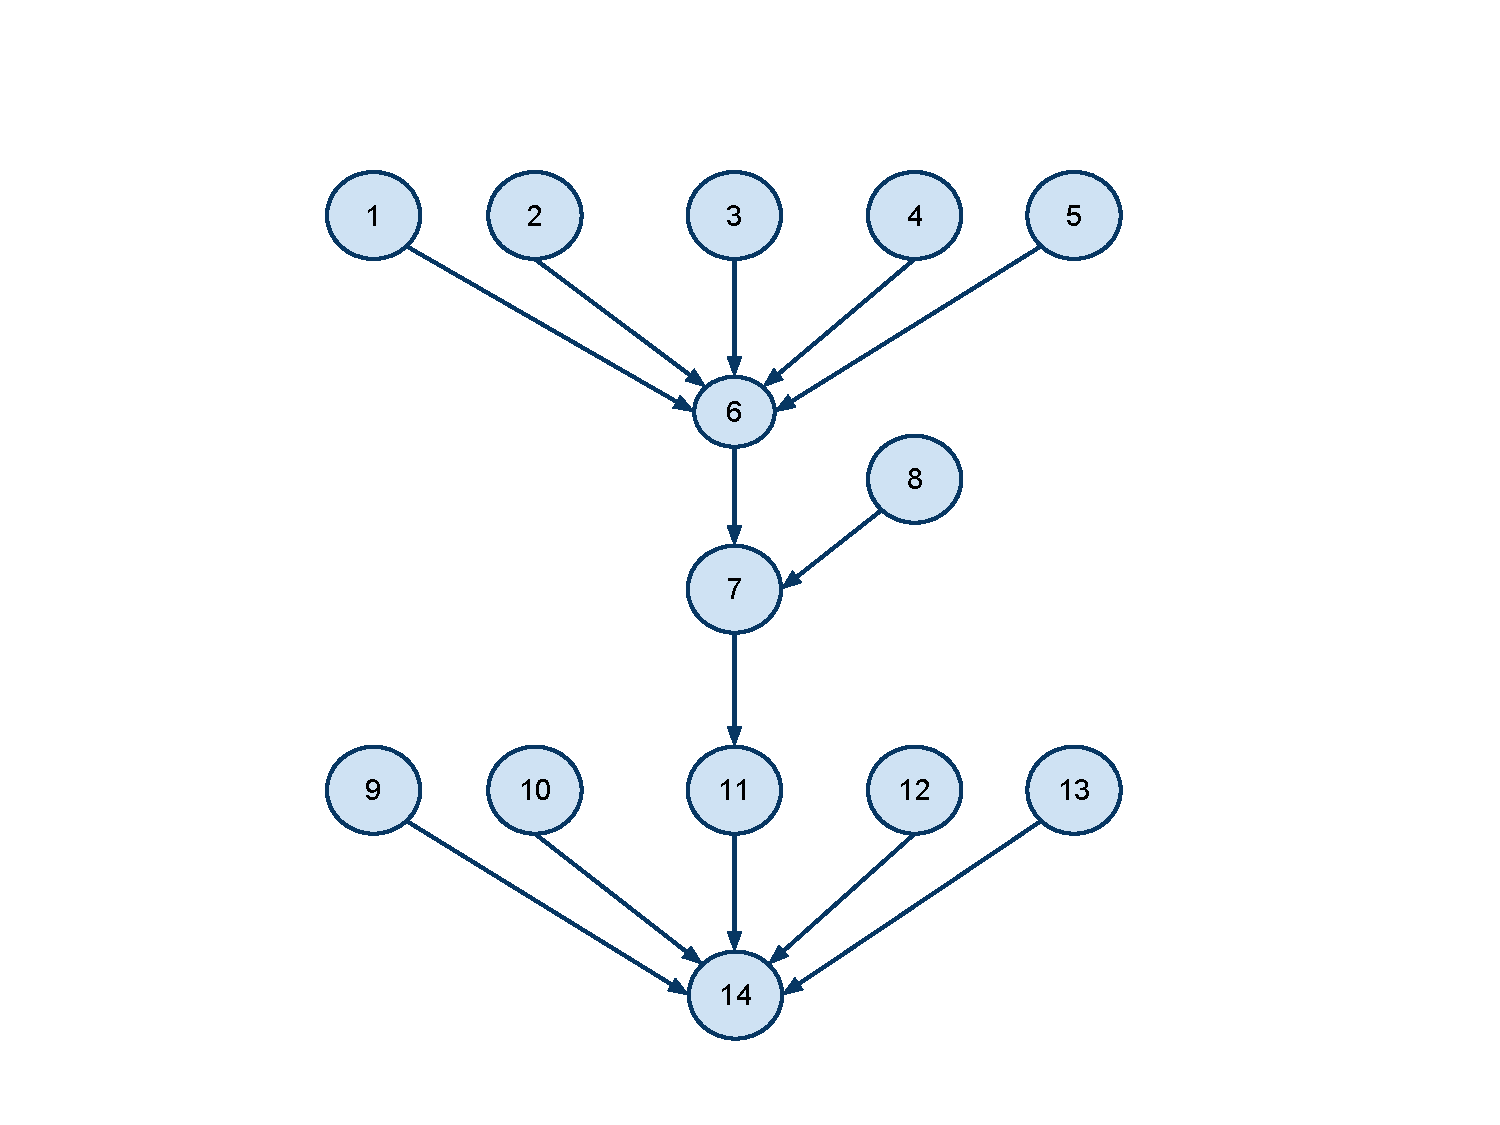
\includegraphics[height=5in]{mq3digraph}
\caption{Task DAG}
\label{fig:dag}
\end{figure}

\begin{enumerate}
\item What is the largest chain in this DAG, if there is more than one, only show one.
\examspace[0.4in]
\item What is the largest antichain? (again, pick one if you find there is more than one).
\examspace[0.4in]
\item How much time would be required to complete all the tasks with a single processor.
\examspace[0.4in]
\item How much time would be required to complete all the tasks if there are unlimited processors available.
\examspace[0.4in]
\item What is the smallest number of processors that would still allow to complete all the tasks in optimal time. Show a schedule proving it.
\examspace[0.4in]
\end{enumerate}

\begin{solution}
\begin{enumerate}
\item One largest chain is $\{1,6,7,11,14\}$
\item One largest antichain is $\{1,2,3,4,5,8,9,10,12,13\}$
\item There are 14 nodes, so a single processor would take 14 seconds.
\item With unlimited processors, we can take 5 seconds. This is the length of the longest chain.
\item With 5 processors, we can still finish everyting in 5 seconds. A schedule showing this
is $\{1,2,3,4,5\}$, $\{6, 8\}$, $\{7\}$, $\{9,10,11,12,13\}$, $\{14\}$. We cannot do this with less than 5 processors 
because in order to make progress on the longest chain at every time step, we need to process $\{1,2,3,4,5\}$ in step 1.
\end{enumerate}
\end{solution}
\end{problem}